\scanpage{27}
\uline{Cas latticiel} : l'intersection de deux facettes fermées est vide, ou une facette fermée.

\uline{Prop.} Pour qu'on soit dans le cas latticiel il f. et s. que a) Pas de ps. droite ! bigonale, et b) pas du type $\mathrm{II}_{4}$

\uline{Proposition} Soit \inserted{$\unsure{\mathcal X|X}$} un arrgt $\overset{\unsure{?}}{2}$-dim de $N$ ps. droites \inserted{$(D_i)_{i\in I}$}, et considérons une \inserted{$(N+1)^{\text{ième}}$} ps. droite $D$ qui ne soit pas bigonale, \inserted{d'où $\mathcal X'$.} Soit $S$ l'ens des sommets sur $D$ \inserted{de $\mathcal X'$}, i.e. l'ens des intersections de $D$ avec les $D_i$ $(i\in I)$. \deleted{Pour tt $s\in S$, soit $\tilde{s}$ \unsure{la facette} de facettes, \unsure{sur $D_i$|pour $(D_i)$}} Pour que \deleted{$s$ et $s'$,} $s,s'\in S$ soient adjacents sur $D$, il f et s. qu'il existe une face fermée $f$ de $\mathcal X$ qui contienne $s$ et $s'$ -- cette face est alors \unsure{uniquemt|unique} déterminée, et $D\cap f$ est un segment joignant $s$ \unsure{à|,} $s'$, tel que $T\cap f=\{s,s'\}$, c'est aussi l'\inserted{unique} arête sur $D$ joignant $s$ et $s'$ \deleted{\unsure{\}}}.
\figure{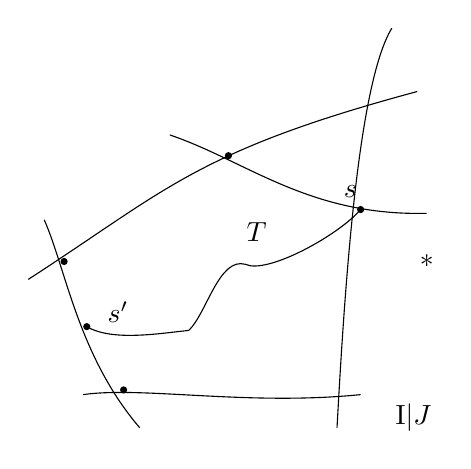
\begin{tikzpicture}[x=.012cm,y=-.012cm]
\draw (5,274) .. controls (152,179) and (183,138) .. (417,75);
\draw (155,121) .. controls (237,149) and (302,207) .. (427,204);
\draw (22,211) .. controls (45,263) and (58,355) .. (123,431);
\draw (63,396) .. controls (126,387) and (237,408) .. (357,396);
\draw (390,8) .. controls (354,67) and (340,284) .. (332,431);
\draw (67,324) .. controls (94,340) and (145,331) .. (175,328) .. controls (194,310) and (207,250) .. (235,258) .. controls (258,269) and (334,227) .. (357,200);
\foreach \x/\y in {67/324,357/200,43/255,217/143,106/391}{\fill (\x,\y) circle[radius=1.3pt];}
\node at (100,309) {$s'$};\node at (346,181) {$s$};\node at (247,224) {$T$};
\node at (413,420) {$\unsure{\mathrm I|J}$};\node at (427,255) {$\unsure{*}$};
\end{tikzpicture}}

\margin{$\mathrm{II}_4\quad\mathrm{II}_5\quad\mathrm{II}_{\unsure{3,2|3,1}},\quad\mathrm{III}_6$}
\deleted{\uline{Lemme} Pour un \unsure{arrangt|arrangement} 1-dim. de $N$ ps. droites sans bigone \inserted{avec $N\geq5$}, on peut trouver \unsure{un arr.} $\mathrm{II}_4$, et une ps. droite $D'$ \unsure{faisant avec celui ci} dans l'un des arrangmts $\mathrm{II}_5,\mathrm{II}_{3,2}$ ou $\mathrm{III}_6$. Quand ensuite on rajoute des ps. droites, elles ne sont jamais bigonales}
% archive sheet number: 26
